%%%%%%%%%%%%%%%%%%%%%%%%%%%%%%%%%%%%%%%%%
% Beamer Presentation
% LaTeX Template
% Version 1.0 (10/11/12)
%
% This template has been downloaded from:
% http://www.LaTeXTemplates.com
%
% License:
% CC BY-NC-SA 3.0 (http://creativecommons.org/licenses/by-nc-sa/3.0/)
%
%%%%%%%%%%%%%%%%%%%%%%%%%%%%%%%%%%%%%%%%%

%----------------------------------------------------------------------------------------
%	PACKAGES AND THEMES
%----------------------------------------------------------------------------------------

\documentclass{beamer}

\mode<presentation> {

% The Beamer class comes with a number of default slide themes
% which change the colors and layouts of slides. Below this is a list
% of all the themes, uncomment each in turn to see what they look like.

%\usetheme{default}
%\usetheme{AnnArbor}
%\usetheme{Antibes}
%\usetheme{Bergen}
%\usetheme{Berkeley}
%\usetheme{Berlin}
%\usetheme{Boadilla}
%\usetheme{CambridgeUS}
%\usetheme{Copenhagen}
%\usetheme{Darmstadt}
%\usetheme{Dresden}
%\usetheme{Frankfurt}
%\usetheme{Goettingen}
%\usetheme{Hannover}
%\usetheme{Ilmenau}
%\usetheme{JuanLesPins}
%\usetheme{Luebeck}
\usetheme{Madrid}
%\usetheme{Malmoe}
%\usetheme{Marburg}
%\usetheme{Montpellier}
%\usetheme{PaloAlto}
%\usetheme{Pittsburgh}
%\usetheme{Rochester}
%\usetheme{Singapore}
%\usetheme{Szeged}
%\usetheme{Warsaw}

% As well as themes, the Beamer class has a number of color themes
% for any slide theme. Uncomment each of these in turn to see how it
% changes the colors of your current slide theme.

%\usecolortheme{albatross}
%\usecolortheme{beaver}
%\usecolortheme{beetle}
%\usecolortheme{crane}
%\usecolortheme{dolphin}
%\usecolortheme{dove}
%\usecolortheme{fly}
%\usecolortheme{lily}
%\usecolortheme{orchid}
%\usecolortheme{rose}
%\usecolortheme{seagull}
%\usecolortheme{seahorse}
%\usecolortheme{whale}
%\usecolortheme{wolverine}

%\setbeamertemplate{footline} % To remove the footer line in all slides uncomment this line
%\setbeamertemplate{footline}[page number] % To replace the footer line in all slides with a simple slide count uncomment this line

%\setbeamertemplate{navigation symbols}{} % To remove the navigation symbols from the bottom of all slides uncomment this line
}

\usepackage{hyperref}
\usepackage{verbatim}
\usepackage{graphicx} % Allows including images
\usepackage{booktabs} % Allows the use of \toprule, \midrule and \bottomrule in tables

%----------------------------------------------------------------------------------------
%	TITLE PAGE
%----------------------------------------------------------------------------------------

\title[Auto Hybrid Generator]{A Framework for an Automatic Hybrid MPI+OpenMP code generation} % The short title appears at the bottom of every slide, the full title is only on the title page

\author{Gustavo Ramirez} % Your name
%\institute[UCLA] % Your institution as it will appear on the bottom of every slide, may be shorthand to save space
%{
%University of California \\ % Your institution for the title page
%\medskip
%\textit{john@smith.com} % Your email address
%}
\date{\today} % Date, can be changed to a custom date

\begin{document}

\begin{frame}
\titlepage % Print the title page as the first slide
\end{frame}

\begin{frame}
\frametitle{Contents} % Table of contents slide, comment this block out to remove it
\tableofcontents % Throughout your presentation, if you choose to use \section{} and \subsection{} commands, these will automatically be printed on this slide as an overview of your presentation
\end{frame}

%----------------------------------------------------------------------------------------
%	PRESENTATION SLIDES
%----------------------------------------------------------------------------------------

%------------------------------------------------
%\section{First Section} % Sections can be created in order to organize your presentation into discrete blocks, all sections and subsections are automatically printed in the table of contents as an overview of the talk
%------------------------------------------------

%\subsection{Subsection Example} % A subsection can be created just before a set of slides with a common theme to further break down your presentation into chunks

%------------------------------------------------
\section{Overview}

\begin{frame}
\frametitle{}

\begin{center}
\textbf{OVERVIEW}
\end{center}

\end{frame}

\begin{frame}
\frametitle{Paper}
\begin{figure}
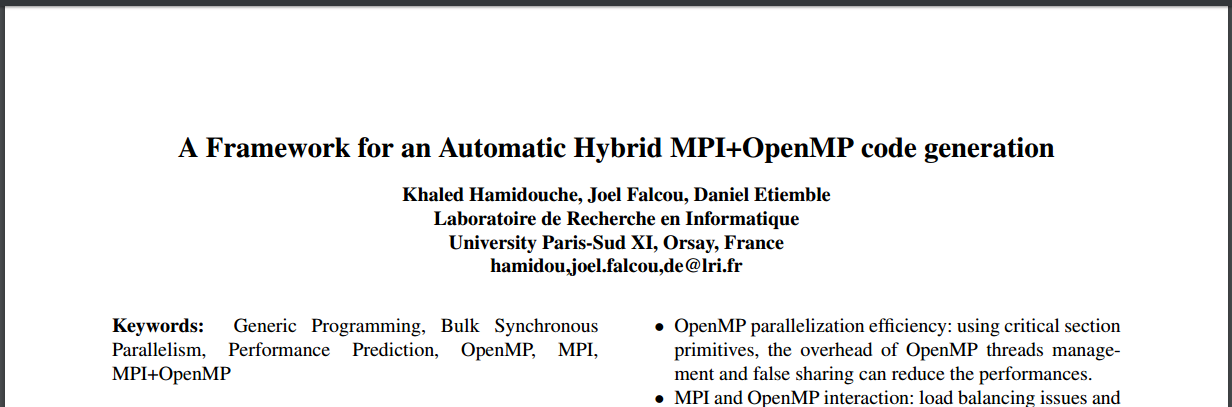
\includegraphics[width=0.8\linewidth]{article-cover}
\end{figure}
\end{frame}

\begin{frame}
\frametitle{General description}

Motivation:

\begin{itemize}
\item writing good hybrid code implies \textbf{expertise} and \textbf{performance analysis}
\item hybrid code can be inefficient (MPI comms overhead, OpenMP critical sects, MPI+OpenMP interaction (e.g. load balancing, idle threads), etc...)
\item $\Rightarrow$ the motivation is not dealing with all that
\end{itemize}

Goal (of this framework): produce efficient hybrid code for multi-core architectures from the source of a sequential function.

\end{frame}

%------------------------------------------------




%------------------------------------------------
\section{Background: BSP + SPMD}

\begin{frame}
\frametitle{}

\begin{center}
\textbf{BACKGROUND}
\end{center}

\end{frame}


\begin{frame}
\frametitle{The BSP model}

BSP model = bulk synchronous parallel model

\ \\


The model is subdivided in:

\begin{itemize}

\item a machine model: 
\begin{itemize}
\item description: set of processors linked through a comm medium supporting point-to-point comms and syncs
\item params: $P$ (nr processors), $r$ (speed, [r] = FLOPS), $g$ (comm speed), $L$ (sync duration)
\end{itemize}
\item a programming model: (see next slide)
\item a cost model: $\delta = W_{max} + hg + L$

\end{itemize}

\end{frame}

\begin{frame}
\frametitle{The BSP model}

\begin{figure}
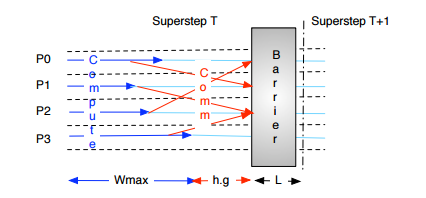
\includegraphics[width=0.8\linewidth]{bsp-description.png}
\end{figure}

$h$: maximal amount of data that is sent or received by one processor

\end{frame}


\begin{frame}
\frametitle{The BSP model}

Cons:

\begin{itemize}
\item cost of global syncs; can become dominant for large parallel machines
\item to reduce the previous problem, use OpenMP to minimize sync overhead
\end{itemize}

Pros:

\begin{itemize}
\item simple analytical model; the BSP cost model facilitates the execution time estimation
\item performance improvement; "best" number of processors and threads
\end{itemize}

\end{frame}


\begin{frame}
\frametitle{SPMD}

Single Program, Multiple Data.

\ \\

Tasks are split up and run simultaneously on multiple processors with different input in order to obtain results faster.

\ \\

Using other mode different from SPMD might imply high thread creation overhead, and serial sections may become bottlenecks. 

\end{frame}

\begin{frame}
\frametitle{SPMD}

Pros:

\begin{itemize}

\item performance prediction is easier (split into Computation and Comm times)
\item avoid false sharing
\item load balancing is good, as all threads execute the same program

\end{itemize}

\end{frame}


%------------------------------------------------




%------------------------------------------------
\section{Implementation: analyzer + searcher + generator}


\begin{frame}
\frametitle{}

\begin{center}\textbf{IMPLEMENTATION}\end{center}

\end{frame}

\begin{frame}
\frametitle{Implementation specs}

Framework specs:

\begin{itemize}

\item uses BSP cost model to estimate exec time
\item finds the best configuration (nr MPI processes + OpenMP threads)
\item generates hybrid code

\end{itemize}

\ \\

Inputs: user source file containing seq code + XML describing parallel code

Outputs: hybrid MPI+OpenMP program

\end{frame}



\begin{frame}
\frametitle{Implementation stages}

Stages: 

\begin{itemize}

\item analyzer: generates a numerical formula for exec time (with data size as param)
\item searcher: uses previous formula and info from the "system profile" to estimate cost for all possible configs
\item generator: uses the chosen configuration and generates the corresponding hybrid code

\end{itemize}

\ \\

System profile: retrieves exec time for basic operations, obtained either from the processor's manual and design specs, or by benchmarking

\end{frame}

\begin{frame}
\frametitle{Analyzer: computation model}

Used to estimate $T_{comm}$. Counts the number of cycles needed to execute a sequential function.

Clang (with all optimizations: -O3) $\rightarrow$ LLVM (which counts the number of cycles in the bytecode).

\ \\

Subdivided:

\begin{itemize}

\item processor model (no cache misses): $total = \sum_{i}C_{i}$, with $C_{i}$ the hardware cost of each operation (e.g. load, store, etc.) $i$
\item cache model (for cache misses): $cost = \sum_{i}^{levels}(M_{i}\cdot PEN_{i})$, with the penalty $PEN_{i}$ given in nr of cycles, and ($j$ represents instructions):

$$M_{i} = \frac{1}{CAPACITY_{i}}\sum_{j}(nr.refs_{i})(\beta_{i})$$

\end{itemize}

\end{frame}

\begin{frame}
\frametitle{Analyzer: communication model}

\begin{itemize}
\item $T_{comm,k} = h_{k}\cdot g_{k}(P_{k}) + L_{k}(P_{k})$, $k\in \{ MPI, OpenMP \}$
\item System profile:
\begin{itemize}
\item combines many benchmarks and sphinx to find $g_{k}(P_{k})$ and $L_{k}(P_{k})$
\item sphinx: tool for running performance tests of MPI, Pthreads and OpenMP
\end{itemize}
\item $T_{comm} = \sum_{k}T_{comm,k}$
\end{itemize}

\end{frame}


\begin{frame}
\frametitle{Searcher: goal}

Uses the XML and the data from the analyzer.

\ \\

Find the best combination number of MPI processes and OpenMP threads.

\ \\

Factors:

\begin{itemize}
\item number of MPI processes
\item number of threads per process
\item data size of the application
\end{itemize}

\end{frame}

\begin{frame}
\frametitle{Searcher: graph}

\begin{figure}
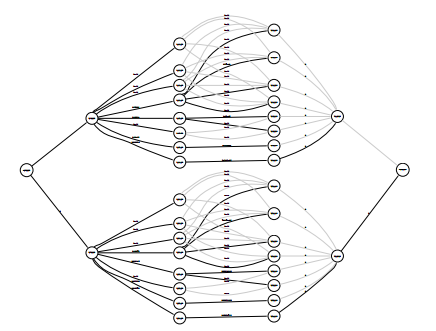
\includegraphics[width=0.5\linewidth]{generator-graph}
\end{figure}

Vertex: $V(S_{i}, n, m, o)$. Edge: $V(S_{i}, n, m, o) \rightarrow V'(S_{i+1}, n, m, o')$.

Use of Dijkstra's shortest path algorithm.

\end{frame}

\begin{frame}
\frametitle{Generator: BSP++ $\rightarrow$ hybrid structure}

\begin{figure}
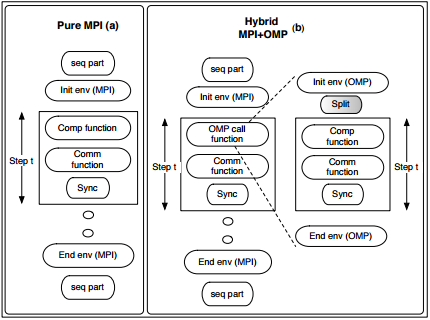
\includegraphics[width=0.8\linewidth]{generator-hybrid-struct}
\end{figure}

\end{frame}


\begin{frame}
\frametitle{Global view}
\begin{figure}
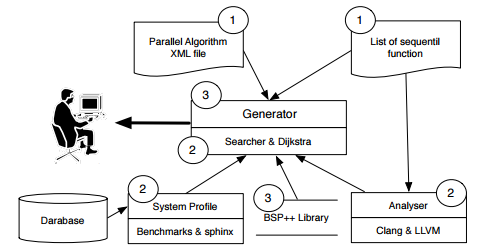
\includegraphics[width=0.8\linewidth]{global-view}
\end{figure}
\end{frame}


%------------------------------------------------




%------------------------------------------------
\section{Results: accuracy + performance}

\begin{frame}
\frametitle{Results: benchmarks and hardware}

Four benchmarks:

\begin{itemize}

\item inner product
\item vector-matrix multiplication
\item matrix-matrix multiplication
\item Parallel Sorting by Regular Sampling algorithm

\end{itemize}

\ \\

Hardware:

4 nodes. Each node is a bi-processor bi-core 2.6 GHz, 4 GB RAM, 2 MB of L2 cache.

\end{frame}


\begin{frame}
\frametitle{Results: model performance}

\begin{figure}
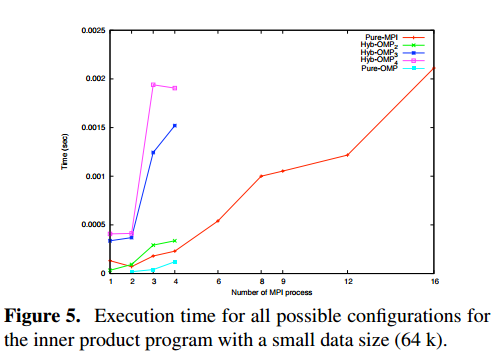
\includegraphics[width=0.8\linewidth]{results-plots1}
\end{figure}

\end{frame}

\begin{frame}
\frametitle{Results: model performance}

\begin{figure}
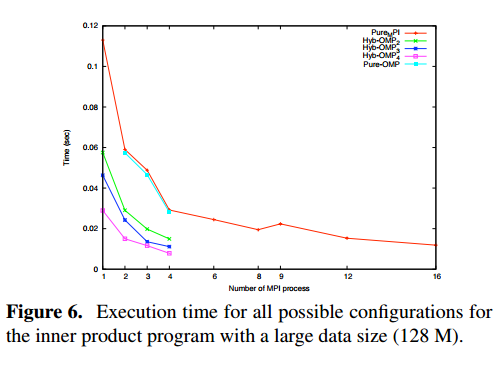
\includegraphics[width=0.8\linewidth]{results-plots2}
\end{figure}

\end{frame}


%------------------------------------------------




\begin{frame}
\frametitle{References}

HAMIDOUCHE, K., FALCOU, J., AND ETIEMBLE, D.
\textit{A Framework for an Automatic Hybrid MPI+OpenMP code generation}. Proceedings of the 19th High Performance Computing Symposia (HPC '11) (2011)

\end{frame}

\begin{frame}
\frametitle{}

\begin{center}
\textbf{Thank you}
\end{center}

\end{frame}






































\begin{comment}

\begin{frame}
\frametitle{What exactly is Machine Learning?}

A lot of things.. and the field is constantly expanding.

\end{frame}

\begin{frame}
\frametitle{What exactly is Machine Learning?}

\textit{"[Machine Learning is the] field of study that gives computers the ability to learn without being explicitly programmed"}

\ \\

First step towards AI...

\ \\

Arthur Lee Samuel (1901-1990): computer gaming, artificial intelligence, machine learning, TeX, ...

\end{frame}


\begin{frame}
\frametitle{What exactly is Machine Learning?}

\textit{"A computer program is said to learn from experience E with respect to some task T and some performance measure P, if its performance on T, as measured by P, improves with experience E."}

\ \\

Tom Mitchell, Carnegie Mellon University

\end{frame}



\begin{frame}
\frametitle{What exactly is Machine Learning?}

\begin{itemize}
\item \textbf{Supervised machine learning}: The program is “trained” on a pre-defined set of “training examples”, which then facilitate its ability to reach an accurate conclusion when given new data.
\item \textbf{Unsupervised machine learning}: The program is given a bunch of data and must find patterns and relationships therein.
\end{itemize}


\end{frame}



\begin{frame}
\frametitle{What exactly is Machine Learning?}

In supervised ML, two major subcategories are:

\begin{itemize}
\item \textbf{regression}: fitting
\item \textbf{classification}: systems where we seek a yes-or-no prediction
\end{itemize}


\end{frame}



\begin{frame}
\frametitle{What exactly is Machine Learning?}
\begin{figure}
%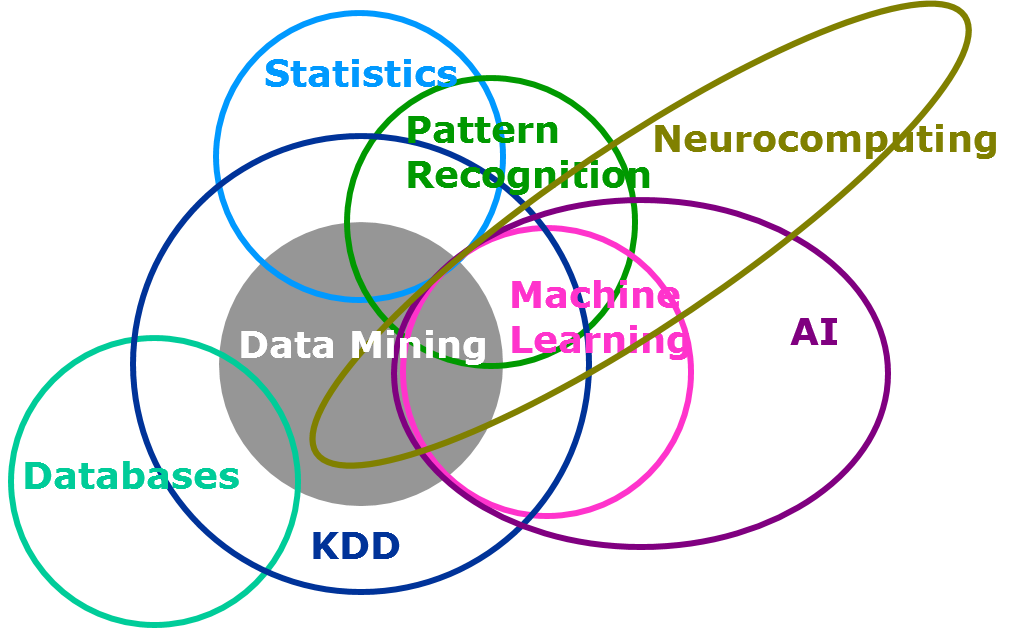
\includegraphics[width=0.8\linewidth]{data-mining-Venn-diagram}
\end{figure}
Image taken from: \hyperref[http://blogs.sas.com/content/subconsciousmusings/2014/08/22/looking-backwards-looking-forwards-sas-data-mining-and-machine-learning/]{''SAS, Data Mining and Machine Learning''}.
\end{frame}




\begin{frame}
\frametitle{What exactly is Machine Learning?}
\begin{figure}
%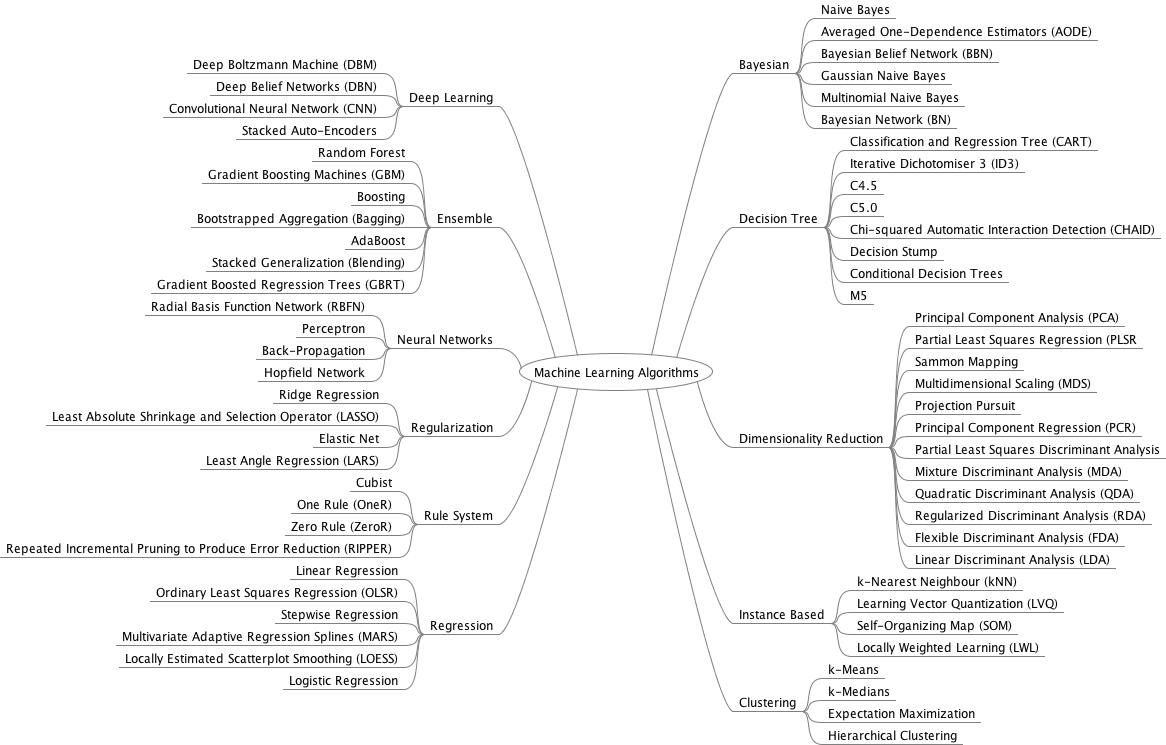
\includegraphics[width=0.9\linewidth]{MachineLearningAlgorithms}
\end{figure}
Image taken from: \hyperref[http://machinelearningmastery.com/a-tour-of-machine-learning-algorithms/]{''A Tour of Machine Learning Algorithms''}.
\end{frame}


%
%


%------------------------------------------------

\section{Multiple Kernel Learning}


\begin{frame}
\frametitle{MKL: meaning}

MKL:

"set of machine learning methods that use a predefined set of kernels and learn an optimal linear or non-linear combination of kernels as part of the algorithm"

\end{frame}



\begin{frame}
\frametitle{MKL: use in SVM}

SVM:

"given labeled training data (supervised learning), the algorithm outputs an optimal hyperplane which categorizes new examples"

\end{frame}


%set of machine learning methods that use a predefined set of kernels and learn an optimal linear or non-linear combination of kernels as part of the algorithm

\begin{frame}
\frametitle{MKL: use in SVM}

\begin{figure}
%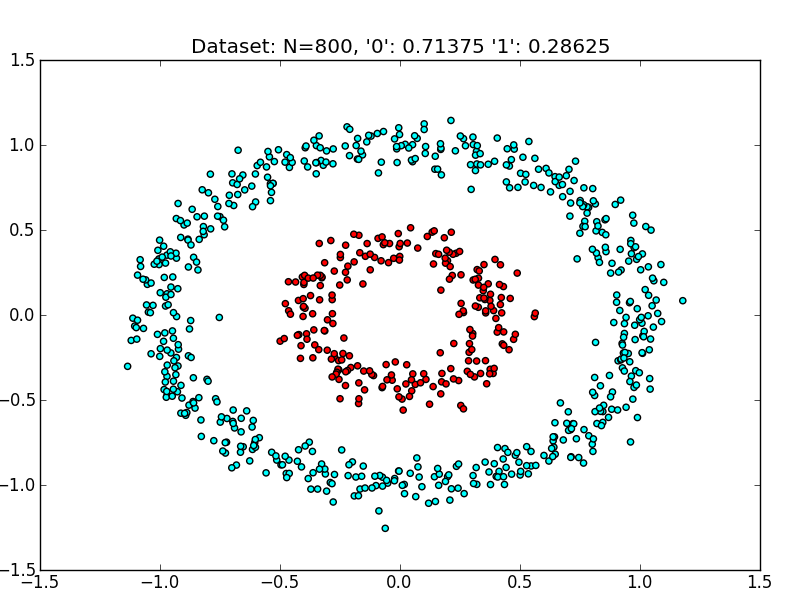
\includegraphics[width=0.9\linewidth]{dataset_nonsep}
\end{figure}
Image taken from: \hyperref[http://www.eric-kim.net/eric-kim-net/posts/1/kernel_trick.html]{''The Kernel Trick''}.

\end{frame}


\begin{frame}
\frametitle{MKL: use in SVM}

The Kernel trick:

\begin{itemize}
\item many ML algorithms (e.g. SVM) use the data only through inner products.
\item e.g. the following matrix (\textbf{kernel matrix}) can be used in classification and regression:
\end{itemize}

\begin{equation}
 X=\begin{bmatrix}
  \vec{x_{1}} \\
  \vec{x_{2}} \\
  ...\\
  \vec{x_{n}}
 \end{bmatrix} \rightarrow 
  K = XX^{T}
\end{equation}

\end{frame}



\begin{frame}
\frametitle{MKL: use in SVM}

The Kernel trick:

\begin{itemize}
\item the idea is to apply a transformation $\phi(\vec{x})$, which preserves the form of $K$:
\end{itemize}

\[
K=
  \begin{bmatrix}
    \phi(\vec{x_{1}})^{T}\phi(\vec{x_{1}}) & \phi(\vec{x_{1}})^{T}\phi(\vec{x_{2}}) & ...  \\
    \phi(\vec{x_{2}})^{T}\phi(\vec{x_{1}}) & ... & ...  \\
    ... & ... & ...
  \end{bmatrix}
\]

\end{frame}


\begin{frame}
\frametitle{MKL: use in SVM}

The Kernel trick:

\begin{itemize}
\item simple example (on a $\phi$ preserving the form of $K$):

\begin{itemize}
\item transformation $\phi$: $(x_{1}, x_{2})\rightarrow (z_{1}, z_{2}, z_{3}) = (x_{1}^{2}, \sqrt{2}x_{1}x_{2}, x_{2}^{2})$
\item let's take: $\vec{r} = \phi(\vec{a})$ and $\vec{s} = \phi(\vec{b})$
\item $\Rightarrow (\vec{r}\cdot\vec{s})_{3D} = r_{1}s_{1}+r_{2}s_{2}+r_{3}s_{3} = (a_{1}^{2})(b_{1}^{2})+(\sqrt{2}a_{1}a_{2})(\sqrt{2}b_{1}b_{2})+(a_{2}^{2})(b_{2}^{2})$
\item $\Rightarrow (\vec{r}\cdot\vec{s})_{3D} = (\vec{a}\cdot\vec{b})^{2}$
\end{itemize}

\item then, the Kernel trick consists of only knowing how to compute the inner product in the new space (through a function of the inner product in the original space), but not the actual transformation
\end{itemize}

\end{frame}



\begin{frame}
\frametitle{MKL: the Kernel trick}

\begin{figure}
%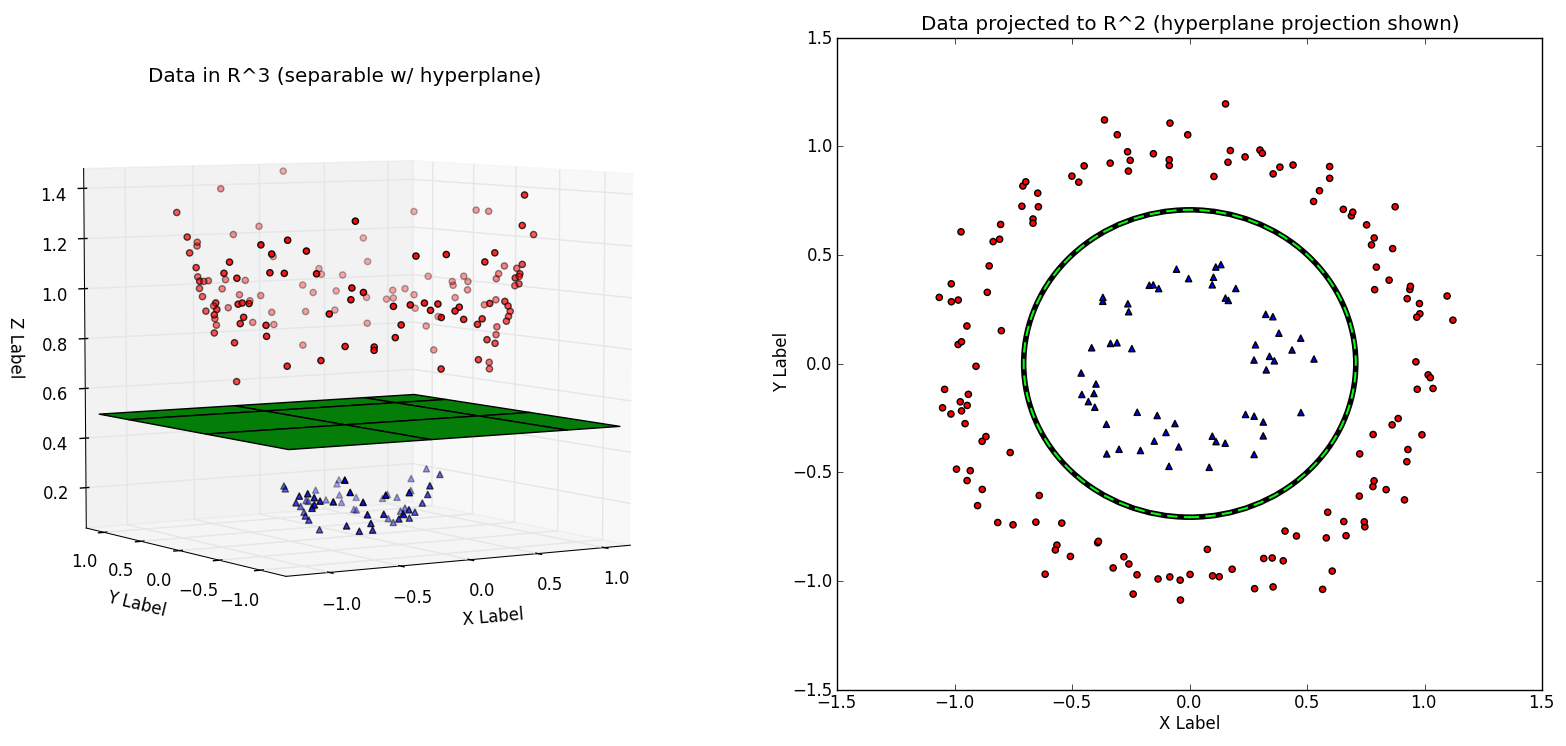
\includegraphics[width=1\linewidth]{data_2d_to_3d_hyperplane}
\end{figure}
Image taken from: \hyperref[http://www.eric-kim.net/eric-kim-net/posts/1/kernel_trick.html]{''The Kernel Trick''}.

\end{frame}



\begin{frame}
\frametitle{MKL: the Kernel trick}

MKL:

\begin{itemize}
\item extension of the Kernel trick, using many $\phi$'s now, and optimize with the original algorithm (SVM or other) but taking those kernels into account
\end{itemize}

\end{frame}





%------------------------------------------------

\section{Applications}

\begin{frame}
\frametitle{Applications of ML}

Prediction in cancer:

\begin{figure}
%
\includegraphics[width=1\linewidth]{article_cancer}
\end{figure}

\end{frame}

\begin{frame}
\frametitle{Applications of ML}

Recommender systems (Netflix, Amazon, etc.), data mining, image recognition, etc.

\end{frame}



%------------------------------------------------

\begin{frame}
\frametitle{References}
\footnotesize{
\begin{thebibliography}{99} % Beamer does not support BibTeX so references must be inserted manually as below

%A community effort to assess and improve drug sensitivity prediction algorithms

\bibitem[Costello, 2006]{p1} James C Costello, \textit{et al.} (2014)
\newblock A community effort to assess and improve drug sensitivity prediction algorithms
\newblock \emph{Nature Biotechnology} 32, 1202–1212 %1531 -- 1565.

\bibitem[Sonnenburg, 2006]{p1} S{\"o}ren Sonnenburg, \textit{et al.} (2006)
\newblock Large Scale Multiple Kernel Learning
\newblock \emph{Journal of Machine Learning Research} 1531 -- 1565.


\end{thebibliography}
}
\end{frame}

%------------------------------------------------

\begin{frame}
\Huge{\centerline{The End}}
\end{frame}

%----------------------------------------------------------------------------------------

\end{comment}


\end{document} 